\section{研究背景与意义}

\subsection{研究背景}
近年来，大语言模型（Large Language Model，LLM）正逐步从被动的的文本生成模型演化为能够主动进行任务规划、工具调用、环境交互和多轮反馈修正的智能体（Agent）。LLM智能体不再局限于从静态提示词生成单一响应，而是能够理解任务上下文、对中间状态进行推理、调用外部工具、检索信息、访问记忆、与环境交互，以及与其他智能体协作\cite{wang2026fromagenttraces}。

在产业实践方面，据Precedence Research统计，2025年全球AI Agent市场规模已达79.2亿美元，预计至2035年将增长至2946.6亿美元，年均复合增长率高达43.57\%；其中企业端应用占比超过67\%，客户服务与虚拟助手、生产效率与个人助理、代码与软件开发等场景构成主要需求驱动力\cite{precedence2025aiagents}。Gartner预测，到2028年将有33\%的生成式AI交互采用Agent式自主决策模式，较2024年的不足1\%实现跨越式增长\cite{gartner2025agentic}。Agent化已掀起2025至2026年人工智能领域的发展热潮，国内外的商业公司涌现出大量应用产品：国际层面包括OpenAI的Agents SDK和Codex、Anthropic的Managed Agents和Claude Code、Google的Project Mariner与Gemini Agent、微软的Copilot Studio及AutoGen\cite{wu2024autogen}、；国内则涵盖阿里巴巴的百炼Agent Builder、字节跳动的Coze平台以及智谱AI的AutoGLM等，共同构筑了百舸争流的市场格局。开源社区方面，以模块化组件库架构著称的LangChain\cite{langchain}、将软件公司标准作业流程映射为多智能体协作的MetaGPT\cite{hong2024metagpt}，以及基于“角色扮演+任务分工”机制的CrewAI等优秀框架相继问世。进入2026年，以OpenClaw为代表的本地优先开源框架开始大规模普及，凭借其多通信渠道支持与可插拔技能系统获得广泛关注；随后的Hermes进一步深化了记忆模块的作用，实现了任务完成后的持续总结与演进。上述商业与开源产品的广泛应用，标志着Agent技术已从学术原型迈向大规模部署阶段。目前，Agent系统已逐步深入办公自动化、软件工程、网络安全运维、数据分析及智能物联网等关键领域\cite{wang2024survey,xi2025rise,park2023generative}，这种深度的产业渗透为随着Agent应用伴生的Agent安全问题研究奠定了坚实的现实基础。

\textbf{从大语言模型到智能体的技术演进。}从技术演进脉络看，面向智能体的大语言模型发展可分为预训练（Pre-training）、适配调优（Adaptation Tuning）与利用（Utilization）三大技术维度\cite{zhao2023survey}，其演进历程可概括为三个关键阶段：\textbf{第一阶段（2017--2019）}是架构奠基与预训练范式确立期，Vaswani等\cite{vaswani2017attention}提出Transformer架构，以自注意力机制取代循环结构，奠定了现代语言模型的计算基础；Radford等\cite{radford2018improving}与Devlin等\cite{devlin2019bert}分别通过GPT-1和BERT验证了预训练-微调范式在语言理解任务上的有效性，确立了语言模型“大规模预训练+任务微调”的基本范式。\textbf{第二阶段（2020--2022）}是规模扩张与能力对齐期，Brown等\cite{brown2020language}推出1750亿参数的GPT-3，首次展示了大语言模型在少样本（Few-shot）场景下的强大泛化能力；Kaplan等\cite{kaplan2020scaling}系统揭示了模型性能与参数量、数据量、计算量之间的幂律缩放关系（Scaling Laws），为后续模型规模扩张提供了可预测的理论依据；Wei等\cite{wei2022emergent}发现当模型参数规模超过特定阈值后，会涌现出小模型不具备的能力，如多步推理、指令遵循和上下文学习，随后据此提出了思维链（Chain-of-Thought，COT）\cite{bosma2022chainofthought}技术，通过在提示词中展示中间推理步骤来激发大型语言模型推理能力，证明了足够大的语言模型在经过少样本CoT提示后，无需微调即可在算术、常识和符号推理任务上取得大幅性能提升；Ouyang等\cite{ouyang2022training}提出InstructGPT，通过指令微调与基于人类反馈的强化学习使模型行为与人类意图对齐，解决了大规模模型“能力强但不可控”的核心矛盾，标志着LLM从能力涌现走向能力可控的关键转折；Schick等\cite{schick2023toolformer}提出的Toolformer探索了模型自监督学习何时调用API、调用何种API以及如何吸收工具返回结果，证明仅需少量标注样本即可使语言模型掌握多种外部工具的使用，从而大幅降低了工具调用能力的训练成本；Wei等\cite{wei2022chain}提出思维链（Chain-of-Thought）提示方法，通过引导模型生成中间推理步骤显著提升多步推理能力，为LLM执行复杂规划任务奠定了推理基础。\textbf{第三阶段（2023至今）}是模型层面的Agent能力集成期，人们对大语言模型的利用维度从文本生成逐渐扩展至Agent式任务执行。OpenAI发布的GPT-4\cite{openai2023gpt4}不仅在多项专业和学术基准上达到人类水平表现，更首次原生支持函数调用（Function Calling）机制，使LLM能够直接生成结构化的工具调用请求并解析返回结果，标志着LLM从文本生成器向任务执行器的技术转变；Gorilla\cite{patil2024gorilla}通过在大规模API语料上微调LLM并使其自主选择并调用真实API，首次验证了LLM可在不依赖人工提示模板的情况下实现高精度工具选择；Qin等\cite{qin2024toolllm}提出的ToolLLM通过构建大规模自动化指令数据集实现了复杂多工具场景的灵活应用，并引入深度优先搜索决策树策略以提升长链工具调用的探索效率与成功率，为开源大模型在真实复杂任务中的工具编排与决策提供了系统化方案；Meta推出的LLaMA\cite{touvron2023llama}和阿里巴巴推出的Qwen\cite{yang2025qwen3technicalreport}系列大模型则使工具调用能力的训练与适配可在开源模型上复现，推动了Agent研究的可复现性与民主化。至此，指令遵循与多步推理能力的涌现与对齐，使得LLM不再仅作为单纯的文本生成器，而是具备了理解任务意图、分解执行步骤并调用外部工具的潜力，这为LLM从语言模型向智能体的角色跃迁奠定了完整的能力基础。

\textbf{基于大语言模型的智能体（Agent）的演化历程。}在\textbf{Agent定义}层面，Wooldridge和Jennings\cite{wooldridge1995intelligent}于1995年从软件智能体角度提出Agent应具备自主性（Autonomy）、社会性（Social Ability）、反应性（Reactivity）和预动性（Pro-activeness）四项核心属性，而Russell和Norvig\cite{russell2020artificial}则于2020年在经典教材《Artificial Intelligence: A Modern Approach》中明确将智能体定义为“通过传感器感知环境并通过执行器作用于环境的实体”。在\textbf{LLM Agent领域}，Weng\cite{weng2023agent}提出了著名的Agent开发公式（Agent=大模型+规划+工具调用+记忆），奠定了现今LLM Agent的形态基础（如\autoref{fig:agent-overview}所示）；Xi等\cite{xi2025rise}将LLM Agent定义为以大语言模型为核心大脑（Brain），结合感知（Perception）与动作（Action）模块，能够在动态环境中自主感知、推理、规划并执行任务的智能体系统，并提出了Brain-Perception-Action三组件通用框架；Wang等\cite{wang2024survey}进一步指出，LLM Agent区别于传统软件智能体的关键在于其以自然语言为统一接口，通过提示词（Prompt）驱动推理与行动，而非依赖预编程规则Masterman等\cite{masterman2024landscape}归纳了AI Agent架构，总结了推理、规划与工具调用三大核心能力的设计范式:推理以思考-行动交织与自反思为主，规划包括任务分解、多计划选择与反思修正等方法，工具调用则围绕单Agent串行（规划、选择与反思）与多Agent分工（职责分离、Agent团队组织）两种模式展开。。而在Agent技术的实践落地层面，Parisi等\cite{parisi2022talm}提出了工具增强语言模型，通过纯文本到文本的API调用格式将外部工具接入语言模型，并设计迭代式“自博弈”机制使模型从少量工具演示中自举学习“何时调用工具及如何构造参数”，证明了工具增强可作为降低语言模型对规模依赖的互补路径；随后，Yao等\cite{yao2023react}提出了ReAct（Reason-Action）提示范式，将推理与行动交织结合，使模型能够交替生成推理轨迹与外部动作（如工具调用），通过与外部环境交互获取实时信息来指导推理与决策过程，有效缓解了纯思维链推理易产生事实幻觉的问题，为LLM向智能体演进提供了早期的交互范式；Shinn等\cite{shinn2023reflexion}则进一步提出了Reflexion机制，旨在通过语言反馈机制使Agent能够从失败经验中学习，将错误调用经验转化为自然语言反思并存入记忆，进一步提升了多步工具调用的鲁棒性与自适应能力；Wang等提出的\cite{wang2024codeact}CodeAct将工具调用动作统一为可执行Python代码，替代传统JSON格式调用，使单次动作即可完成多步操作与条件分支，在减少交互轮次的同时并显著提升了任务完成率。这些工作开始让大语言模型突破传统文本生成的形态限制，让LLM不再仅依赖内部参数完成推理，而是通过外部API、检索系统、文件系统、邮件日程、数据库、浏览器或代码执行器等工具获取信息并改变外部环境，成为与环境交互甚至嵌入环境本身的实体。在\textbf{多Agent协作}层面，Qian等\cite{qian2024chatdev}提出ChatDev，以“首席执行官（CEO）—首席技术官（CTO）—程序员—测试员”等软件公司角色链驱动多Agent对话式协作完成软件开发，验证了角色分工式对话在代码生成任务上的可行性；Wu等\cite{wu2024autogen}提出AutoGen框架，将Agent抽象为可定制、可对话的实体，支持LLM推理、人类输入和工具调用的灵活组合模式，允许开发者通过自然语言与代码混合编程定义Agent间的多轮对话拓扑、自动回复策略和人工介入条件，使得多Agent系统的编排从手工硬编码转向声明式配置，已被广泛应用于数学推理、代码生成和运营决策等场景；Hong等\cite{hong2024metagpt}提出MetaGPT框架，将软件公司的标准作业流程（Standard Operating Procedure, SOP）编码为提示序列，定义产品经理、架构师、工程师和QA工程师等多重角色，通过共享消息池与发布-订阅机制实现结构化通信，Agent间以文档和图表等结构化产出物而非自由对话进行交接，验证了SOP驱动的多Agent系统在复杂软件工程任务上的有效性。然而，上述框架在设计时均以任务完成率为核心优化目标，缺乏对工具调用链的过程级安全审计机制——ChatDev的纯对话式协作使注入内容可在角色间无约束传播，AutoGen的灵活对话拓扑意味着恶意Agent可通过多轮对话逐步提升权限，MetaGPT的结构化SOP虽降低了幻觉风险但未对跨角色数据流进行安全隔离，这些安全缺口的客观存在正是本研究所关注的问题。自动程序从“规则驱动”到“语言驱动”的范式转变，正是LLM Agent安全问题的根源所在：当智能体的行为由语义而非语法决定时，传统的访问控制与权限管理机制将面临根本性的适用性挑战\cite{chu2026systematic}。


\begin{figure}[htbp]
  \centering
  \resizebox{\textwidth}{!}{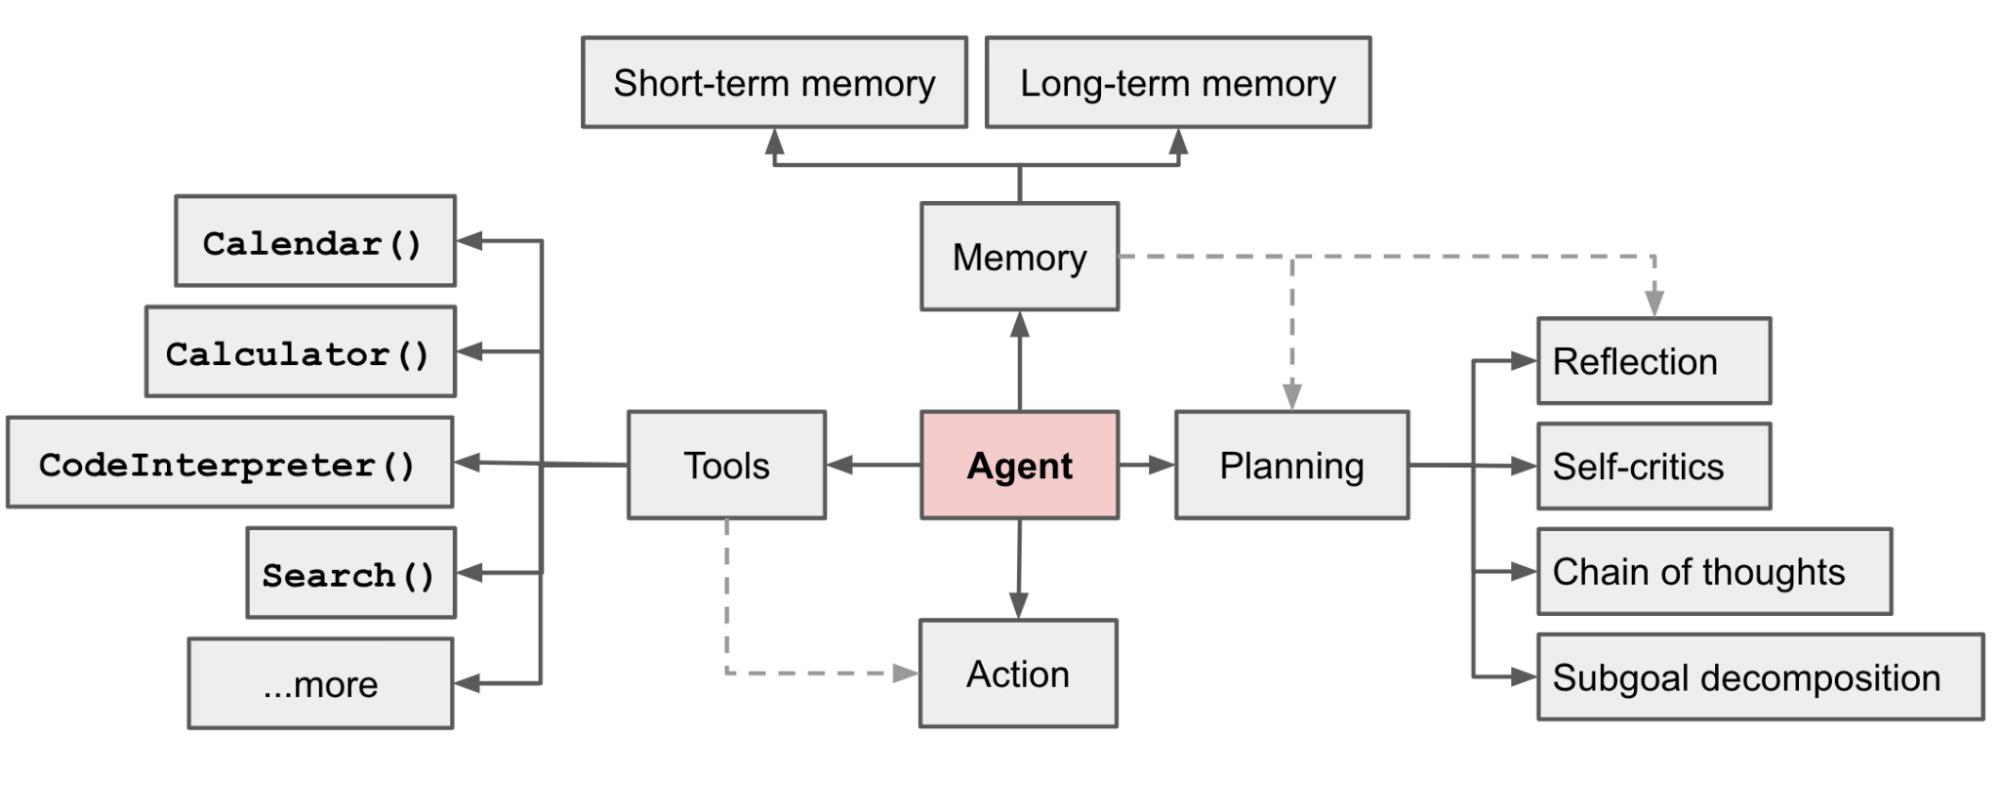
\includegraphics{figures/agent-overview.png}}
  \caption{Lilian Weng\cite{weng2023agent}提出的Agent开发公式}
  \label{fig:agent-overview}
\end{figure}

\textbf{工具调用型Agent带来的新型安全威胁。}LLM Agent的工具调用能力在显著拓展其任务边界的同时，也引入了区别于传统模型安全的全新攻击面。Greshake等\cite{greshake2023nowwhat}于2023年首次揭示的间接提示注入（Indirect Prompt Injection，IPI）威胁，从根本上了暴露工具调用场景中“数据—指令边界模糊”这一结构性安全缺陷；随后，早期的安全评估基准\cite{balunovic2024agentdojo,ruan2024toolemu}开始将安全评估从模型内部的响应级扩展至Agent与外部世界交互的行为级。随着工具数量激增与调用链日趋复杂，攻击向量迅速从内容注入向工具全生命周期扩散：在工具选择与权限维度，攻击者可劫持工具选择决策或诱导越权调用\cite{shi2026pitoolselection,zhang2026evaluatingprivilege,jha2026agent}；在供应链维度，技能投毒与多工具组合攻击揭示了跨步骤隐式风险的存在\cite{tie2026badskill,wu2026chainfuzzer}。包括提示/内容注入、工具滥用/投毒等攻击向量已被认为成为Agent安全的独立核心威胁面，且多向量组合攻击的威胁等级远超单点攻击\cite{deng2025agentsunderthreat,dehghantanha2026sokattacksurfaceagentic}。面对日益严峻的安全形势，学界先后探索了以架构级隔离寻求确定性安全保证\cite{debenedetti2025camel,costa2025fides,wu2025isolategpt}、以步骤级护栏与依赖图建模实现运行时动态拦截\cite{mou2026toolsafe,an2025ipiguard}、以协议强制与执行溯源将防御目标从阻止攻击延伸至感知与追溯\cite{uppala2026prompts,wang2026fromagenttraces}等递进的三层防御范式。

然而，尽管上述工作在攻击发现与单点防御方面取得了重要进展，现有研究仍存在若干结构性不足，构成当前领域的核心研究缺口：其一，\textbf{当前防御范式以“安全/不安全”的二元判定为主导}，缺乏对工具调用链执行过程的细粒度、可解释风险度量。单次工具调用的安全风险并非单纯的二进制属性，而是由工具敏感性、权限边界、调用深度、操作不可逆性及人工确认介入程度等多维因素共同决定的连续值，二元分类既无法区分“高风险但可逆”与“中等风险但不可逆”两种本质不同的威胁情境，亦无法为运维人员提供可操作的归因信息。其二，\textbf{多数防御方案在单步工具调用层面操作，对跨步骤风险的路径级组合效应缺乏感知能力}现有研究已经表明，大量Agent漏洞需要多工具路径方能触发\cite{wu2026chainfuzzer}，子任务单独良性但组合后形成有害行为的分解攻击难以被单步检测机制捕获\cite{kothamasu2026hidden}，这一“组合性安全缺口”正是本研究的核心关切所在。其三，\textbf{现有防御普遍聚焦于“阻止攻击发生”而忽视了“感知攻击发生并追溯根源”的能力}，缺乏面向Agent全生命周期（部署前评估、运行时检测、事后审计归因）的感知—防御一体化框架，使得安全运维人员即便部署了防御措施，仍无法系统性回答“风险存在于哪些调用环节”“攻击是否正在发生”“攻击是如何发生的”等关键运维问题。

综合上述背景，LLM Agent在现代AI产业体系中正在占据越来越重要的生态位，而Agent工具调用链的安全问题正是其中的关键挑战；而针对LLM Agent的工具调用链的威胁归因与防御方法研究，正是弥合这一安全缺口的必要举措。本研究致力于提出一种可解释的风险度量体系，并据此设计轻量级的防御中间件，为LLM Agent工具调用的可解释安全性保障提供理论支撑和工程实践指导。

\subsection{研究意义}

\subsubsection{理论意义}

\begin{enumerate}
  \item 本研究从工具调用链出发，将Agent安全问题由“输入输出文本安全”扩展到“过程级行为安全”，提出可解释风险度量体系，将工具敏感性、权限边界、调用深度、不可逆性和人工确认等因素纳入统一框架，对工具调用链的组合性威胁风险进行分级量化和防御；在单工具调用链风险度量的基础上，进一步将Agent执行过程中的工具上下文元素之间的依赖关系进行形式化图表达，为工调用链风险检测和归因提供结构化基础，有助于弥补现有研究中“重防御结果、轻过程感知”的不足。

  \item 本研究将系统安全领域的溯源图思想\cite{inam2023sok,gao2021threatraptor,cheng2024kairos}迁移至LLM Agent场景，提出适应Agent执行语义的异构轨迹图表示，为Agent可观测性和执行溯源研究提供新的方法论视角，从而为Agent安全从“攻防对抗”向“过程审计、威胁归因”的防御范式演进提供一种可能的思路，以弥补现有工作在跨步骤风险路径识别、可解释威胁归因和最小干预防御方面的局限性。
\end{enumerate}

\subsubsection{实用价值}

\begin{enumerate}
  \item 从框架贡献角度看，本研究构建的低成本可复现任务集与评估框架，可为后续Agent安全研究提供标准化的实验基座，降低研究门槛，促进该方向的可复现性和可比较性。
  
  \item 从工程落地角度看，本研究旨在设计一个轻量级、可接入现有LLM Agent系统的的可插拔审计模块，接收Agent执行日志，输出工具调用链风险分数、异常模式、关键风险路径和归因报告。对于企业办公Agent、数据分析Agent、代码执行Agent和Agentic IoT原型系统而言，该审计模块可以作为部署前评估、运行时监控和事后审计的轻量组件，回应了OWASP LLM Top 10威胁\cite{owasp2025llmtop10}对工具调用安全审计工具的明确需求。
\end{enumerate}

\subsubsection{与国家及行业发展战略的契合度}

\begin{enumerate}
  \item 契合《新一代人工智能发展规划》中关于“人工智能安全”的战略部署，为AI系统的安全评估与风险防控提供关键技术支撑。
  \item 响应《网络安全法》和《数据安全法》对关键信息基础设施安全保护的要求，为LLM Agent在金融、政务等敏感领域的安全部署提供风险度量与审计方法。
  \item 服务于国家人工智能标准化总体组关于“人工智能可信特征”标准的研究，为LLM Agent工具调用链的安全性与可解释性评测以及对应的风险防御提供方法论参考。
\end{enumerate}
